% $Id: results.tex 
% !TEX root = ../main.tex

\section{Analysis and Results}
\label{sec:results}

This section presents the analysis of the results of the empirical study presented in 
\fref{sec:evaluation}. The results are presented according to three sections in the survey: General 
knowledge (\fref{sec:general-knowledge}), Task Effectiveness (\fref{sec:tasks-results}) and usability 
(\fref{sec:usability}). Additionally, a discussion section is added analyzing the results form the survey. 
All data obtained from the evaluation is available as part of the data and replication 
package.


%%
\subsection{General Knowledge Results}
\label{sec:general-knowledge}

Most of the participants were very experienced with programming in Python as it can be seen in 
(\fref{fig:python-experience}). The experience level of 5 is selected as participants use Python very 
often in their work and university courses. 
Similarly, most participants are well familiarized with \ac{RL} (\fref{fig:rl-experience}), as they were 
taking a course on the topic. This is very important information, as the bugs required familiarity with 
\ac{RL} and Python knowledge to be identified. Furthermore, the participants report being familiar 
with using the terminal, and therefore, interacting with \flik, using the commands and the interface 
would not pose a problem or require a learning curve (\fref{fig:terminal-experience}). 
Nevertheless, in average, the participants were not familiarized with debuggers, and only used them  
rarely, normally using Visual Studio Code interface's simple features, like graphical breakpoint 
functionality. This lead to misunderstandings and some difficulties in completing the tasks, as the 
tool is based on command line interaction to stop and step through the code 
(\fref{fig:debugging-experience}). This characteristic from the participants caused a steeper learning 
curve to use the tool, than expected from participants with previous debugger experience.

In all the graphs in \fref{fig:general-know} the y-axis represents the number of participant  
responses for each question for a particular score in the Likert scale, and the x-axis represents score, 
between 5 and 1 (from completely agree to completely disagree).

\begin{figure}[hptb]
    \centering
    \begin{subfigure}[b]{0.45\textwidth}
        \centering
        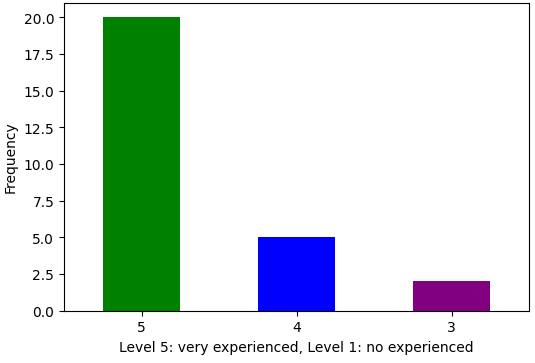
\includegraphics[width=\textwidth]{figures/experience-python}
        \caption{Experience using Python}
        \label{fig:python-experience}
    \end{subfigure}
    ~ 
    \begin{subfigure}[b]{0.45\textwidth}
        \centering
        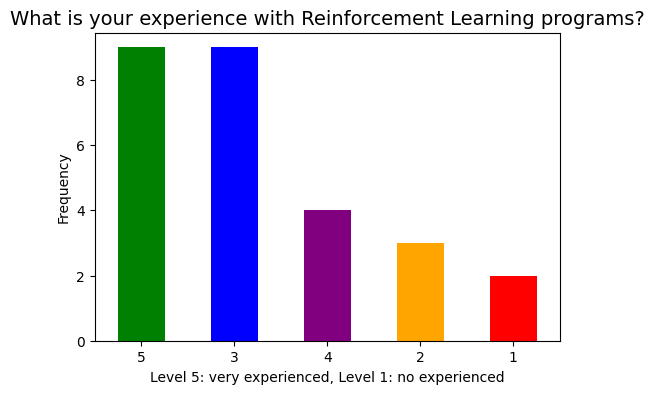
\includegraphics[width=\textwidth]{figures/experience-rl}
        \caption{Experience in \ac{RL}}
        \label{fig:rl-experience}
    \end{subfigure}
    ~ 
    \begin{subfigure}[b]{0.45\textwidth}
        \centering
        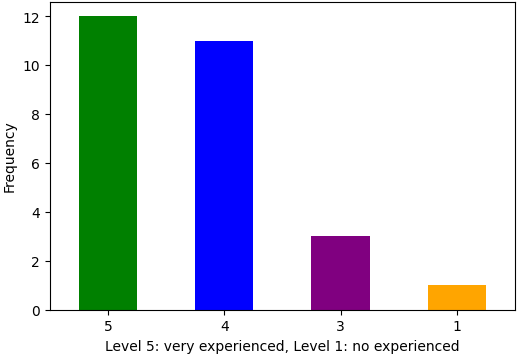
\includegraphics[width=\textwidth]{figures/experience-terminal}
        \caption{Experience using the terminal}
        \label{fig:terminal-experience}
    \end{subfigure}
    ~ 
    \begin{subfigure}[b]{0.45\textwidth}
        \centering
        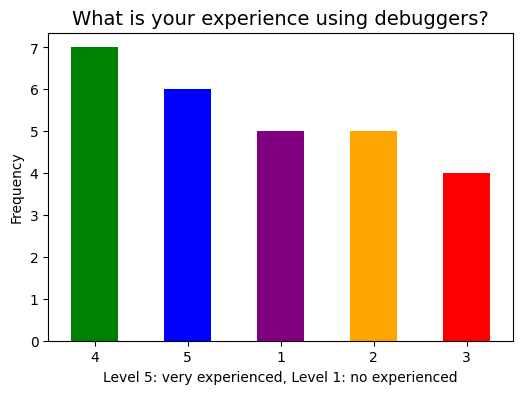
\includegraphics[width=\textwidth]{figures/experience-debuggers}
        \caption{Experience in debugging}
        \label{fig:debugging-experience}
    \end{subfigure}
    \caption{Experience reported by users in the four main dimensions of the tools used in the evaluation}
    \label{fig:general-know}
\end{figure}


%%
\subsection{Tasks Results}
\label{sec:tasks-results}

Taking the results reported from the three tasks, most of the participants completed the first task 
successfully (\fref{fig:task1}). Participants reported the task was easy to solve. Even though the task 
was reported to be easy, it took participants a long time to complete, because this was the task in 
which participants had to get familiarized with the tool. The second task was harder than the first one, 
as participant were not familiar with the problem, and its complexity is higher. Most participants took 
longer to finish task2 (\fref{fig:task2}), and struggled finding the root cause of the bug in the program. 
Such result is expected, as the bug introduced in task 2, does not exhibit a completely wrong agent 
behavior, but a more subtle interaction with the environment and the obtained Q-values. Moreover, the 
fix required more than updating a value, but actually modifying the learning function. Such required 
changed confused many of participants. Finally, the third task (\fref{fig:task3}) was the hardest 
task, most participants had trouble finding the bug. The general comments about the task is that it 
was not easy to solve. Nevertheless, the participants managed to finish the task in less time than in 
the other tasks. 

From the results it is expected that identifying and fixing the bug in the first task take longer than for 
other tasks, even though this is the easiest task, participants are still getting familiarized with the tool, 
and the learning curve for debugging the programs is steep. In the following tasks, while the nature of 
the introduced bugs is different, there is a learning curve  with using the tool. For the second task,
given the nature of the bug and the fact that the bug was introduced in the Q-learning algorithm's 
logic, it was harder to identify. Hence, this task was harder to solve, even though was completed by 
most participants. Finally, for the third task, the introduced bug had yet a different nature, in the 
reward function. For this tasks the learning curve in using the tool was more developed, and it took 
participants less time than expected for this reason.

In \fref{fig:general-know} the y-axis represents the number of participants registering 
answers to the question at the given Likert score. The x-axis corresponds to the score, with
values in the range from 5 to 1 (from completely agree, to completely disagree). In the last 
question (the third bar in green for all graphs), 5 represents taking a lot of time, and 1 represents 
taking very little time.

\begin{figure}[hptb]
    \centering
    \begin{subfigure}[b]{0.32\textwidth}
        \centering
        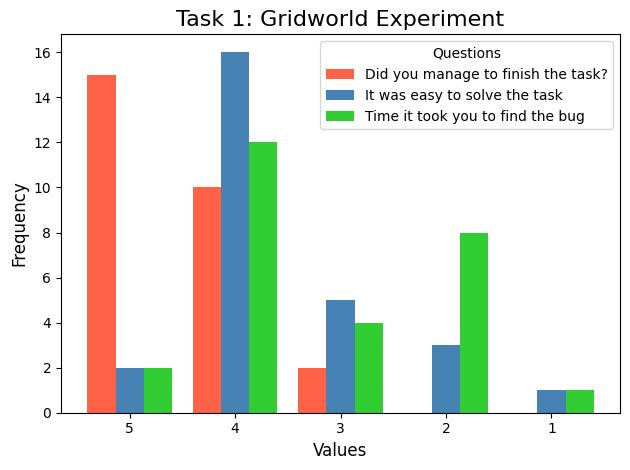
\includegraphics[width=\textwidth]{figures/task1}
        \caption{Gridworld task}
        \label{fig:task1}
    \end{subfigure}
    ~ 
    \begin{subfigure}[b]{0.32\textwidth}
        \centering
        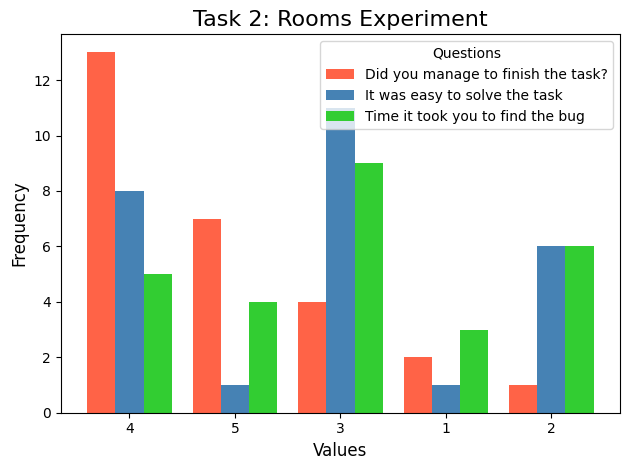
\includegraphics[width=\textwidth]{figures/task2}
        \caption{Rooms task}
        \label{fig:task2}
    \end{subfigure}
    ~ 
    \begin{subfigure}[b]{0.32\textwidth}
        \centering
        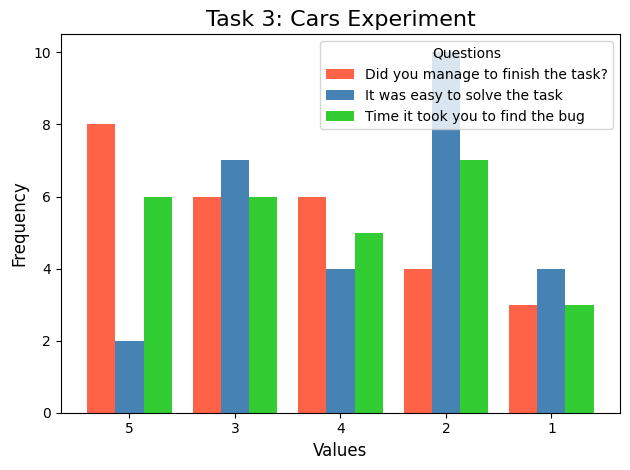
\includegraphics[width=\textwidth]{figures/task3}
        \caption{Cars task}
        \label{fig:task3}
    \end{subfigure}
    \caption{Results of the tasks to solve}
    \label{fig:general-know}
\end{figure}


%%
\subsection{Debugger Usability Results}
\label{sec:usability}

The results for  the debugger's usability, shown in \fref{tab:general1-debuggers} and 
\fref{tab:general2-debuggers}, exhibit a sense that the tool is useful. The comments, in general,  
express that \flik would be useful, specially if given more time to study it, and gain practice with the 
tool before using it in real tasks. The tool was easy to use, once familiarized with the commands and 
their use. Additionally, there are several comments about providing a GUI or improving the current UI,
to help understanding how the tool works, and how to navigate the code with it, as at it differs from 
more mainstream debuggers like the one available with Visual Studio Code and its interface.

\begin{table}[H]
  \centering
  \caption{General Results Part 1}
  \resizebox{\columnwidth}{!}{%
\begin{tabular}{c | *{5}{>{\centering\arraybackslash}p{5cm}}} 
  & \textbf{I have found too much inconsistency in this system} 
  & \textbf{I think most people would learn to use the system quickly} 
  & \textbf{I found the system quite awkward to use} 
  & \textbf{I have felt very safe using the system} 
  & \textbf{I would need to learn a lot of things before I could handle the system} \\
\toprule
\textbf{5} & {1}   & {7}  & {4}  & {7}   & {8.0}                                                                                                                        \\
\textbf{4} & {2}                                                                                                      & {6}                                                                                                             & {7}                                                                                           & {8}                                                                                          & {6.0}                                                                                                                        \\
\textbf{3} & {4}                                                                                                      & {6}                                                                                                             & {9}                                                                                           & {7}                                                                                          & {4.0}                                                                                                                        \\
\textbf{2} & {7}                                                                                                      & {6}                                                                                                             & {4}                                                                                           & {4}                                                                                          & {0.0}                                                                                                                        \\
\textbf{1} & {13}                                                                                                     & {2}                                                                                                             & {3}                                                                                           & {1}                                                                                          & {9.0}                                                                                                                       
\end{tabular}%
}

  \label{tab:general1-debuggers}
\end{table}

\begin{table}[H]
  \centering
  \caption{General Results Part 2}
  \resizebox{\columnwidth}{!}{%
\begin{tabular}{ c |  *{5}{>{\centering\arraybackslash}p{4cm}}}
% \multicolumn{6}{c}{\cellcolor[HTML]{FFFFFF}{ \textbf{Task 2: Rooms Experiment.}}}                                                                                                                                                                                                                                                                                                                                                                                                                                                                                                                                                                                      \\
 & \textbf{I think I would like to use this system frequently} 
 & \textbf{I find this system unnecessarily complex}
 & \textbf{I think the system is easy to use}
 & \textbf{I think I would need technical support to use the system} 
 & \textbf{I find the various functions of the system quite well integrated} \\
 \toprule
\textbf{5} & { 7}                                                                                                      & { 2}                                                                                            & { 5}                                                                                   & { 9}                                                                                                            & { 6}                                                                                                                    \\
\textbf{4} & { 5}                                                                                                      & { 7}                                                                                            & { 5}                                                                                   & { 8}                                                                                                            & { 13}                                                                                                                   \\
\textbf{3} & { 7}                                                                                                      & { 7}                                                                                            & { 11}                                                                                  & { 4}                                                                                                            & { 5}                                                                                                                    \\
\textbf{2} & { 7}                                                                                                      & { 6}                                                                                            & { 6}                                                                                   & { 3}                                                                                                            & { 2}                                                                                                                    \\
\textbf{1} & { 1}                                                                                                      & { 5}                                                                                            & { 0}                                                                                   & { 3}                                                                                                            & { 1}                                                                                                                   
\end{tabular}%
}

  \label{tab:general2-debuggers}
\end{table}

% \begin{table}[]
% \centering
%  \resizebox{\columnwidth}{!}{%
 \begin{tabular}{ c | *{5}{>{\centering\arraybackslash}p{3cm}}}
 \multicolumn{11}{c}{\cellcolor[HTML]{FFFFFF}{ \textbf{Debugger Usability.}}}                                                                                                                                                                                                                                                                                                                                                                                                                                                                                                                                                                                                                                                                                                                                                                                                                                                                                                                                                                                                                                                                                                                                                                                                                                                         \\
 { \textbf{}}  & { \textbf{\begin{tabular}[c]{@{}c@{}}I think I would like to use this \\ system frequently\end{tabular}}} & { \textbf{\begin{tabular}[c]{@{}c@{}}I find this system \\ unnecessarily complex\end{tabular}}} & { \textbf{\begin{tabular}[c]{@{}c@{}}I think the system \\ is easy to use\end{tabular}}} & { \textbf{\begin{tabular}[c]{@{}c@{}}I think I would need technical \\ support to use the system\end{tabular}}} & { \textbf{\begin{tabular}[c]{@{}c@{}}I find the various functions of the \\ system quite well integrated\end{tabular}}} & { \textbf{\begin{tabular}[c]{@{}c@{}}I have found too much \\ inconsistency in this system\end{tabular}}} & { \textbf{\begin{tabular}[c]{@{}c@{}}I think most people would learn \\ to use the system quickly\end{tabular}}} & { \textbf{\begin{tabular}[c]{@{}c@{}}I found the system quite \\ awkward to use\end{tabular}}} & { \textbf{\begin{tabular}[c]{@{}c@{}}I have felt very safe \\ using the system\end{tabular}}} & { \textbf{\begin{tabular}[c]{@{}c@{}}I would need to learn a lot \\ of things before I could handle the system\end{tabular}}} \\
 { \textbf{5}} & { 7}                                                                                                      & { 2}                                                                                            & { 5.0}                                                                                   & { 9}                                                                                                            & { 6}                                                                                                                    & { 1}                                                                                                      & { 7}                                                                                                             & { 4}                                                                                           & { 7}                                                                                          & { 8.0}                                                                                                                        \\
 { \textbf{2}} & { 7}                                                                                                      & { 6}                                                                                            & { 6.0}                                                                                   & { 3}                                                                                                            & { 2}                                                                                                                    & { 7}                                                                                                      & { 6}                                                                                                             & { 4}                                                                                           & { 4}                                                                                          & { 0.0}                                                                                                                        \\
 { \textbf{3}} & { 7}                                                                                                      & { 7}                                                                                            & { 11.0}                                                                                  & { 4}                                                                                                            & { 5}                                                                                                                    & { 4}                                                                                                      & { 6}                                                                                                             & { 9}                                                                                           & { 7}                                                                                          & { 4.0}                                                                                                                        \\
 { \textbf{4}} & { 5}                                                                                                      & { 7}                                                                                            & { 5.0}                                                                                   & { 8}                                                                                                            & { 13}                                                                                                                   & { 2}                                                                                                      & { 6}                                                                                                             & { 7}                                                                                           & { 8}                                                                                          & { 6.0}                                                                                                                        \\
 { \textbf{1}} & { 1}                                                                                                      & { 5}                                                                                            & { 0.0}                                                                                   & { 3}                                                                                                            & { 1}                                                                                                                    & { 13}                                                                                                     & { 2}                                                                                                             & { 3}                                                                                           & { 1}                                                                                          & { 9.0}                                                                                                                       
 \end{tabular}%
 }

% \end{table}

In Tables \ref{tab:general1-debuggers} and \ref{tab:general2-debuggers} the scale represents the 
Likert score option, expressing whether the participants completely agree ($5$) or completely disagree 
($1$) with he question at hand. The values inside the tables correspond to the number of participants 
that reported each given scale.

%%
\subsection{Discussion}
\label{sec:discussion}

In general, the results of the empirical evaluation are very positive. Most of the participants have a 
good impression of \flik, finding it to be useful, specially for the kind of challenges presented in 
\ac{RL} programs. While participants found it hard to familiarize themselves with the tool, specially 
for the participants with little experience with debuggers, at the beginning at the evaluation session, 
most of the participants found the tool easy to use (after some initial use). Additionally, participants 
mention the tool be of use in general for the development of \ac{RL} programs in general, for example 
to develop course work, identifying the errors in the study as recurrent during development. the 
participants to the empirical study highlight \textbf{\flik is useful in detecting common and hard to 
identify errors and miss behavior in \ac{RL} programs}.

With respect to the usability dimension the participants reported that, with some difficulties at the 
beginning, again for the participants without previous experience with debuggers, 
\textbf{\flik is usable}. The usability of the tool is confirmed by the completion of the three tasks by a 
majority of the participants, and the rapid learning curve gathered when switching between tasks, 
reaching a faster and more fluent code navigation to inspect the program, identify the cause of the 
error, and fix the bug, as reported in the time taken to complete each task. Nonetheless, the 
participants note that to increase the usability of \flik \textit{it is desirable to implement more GUI 
features closer to common features used in other debuggers, as the Visual Studio Code debugger}.


\endinput

